\section{Symmetric monoidal double categories}
\label{sec:symm-mono-double}

In this section, we recall basic notions of double categories to fix our terminology and notation, and define monoidal double categories and functors between them in an explicit way.
Double categories go back originally to Ehresmann
in~\cite{ehresmann:cat-str}; a brief introduction can be found
in~\cite{ks:r2cats}.  Other references
include~\cite{multi_funct_i,gp:double-limits,gp:double-adjoints,aleiferi2018cartesian}.


\begin{defn}\label{def:dblcat}
  A \textbf{(pseudo) double category} \lD\ consists of a `category of
  objects' $\lD_0$ and a `category of arrows' $\lD_1$, with structure
  functors
  \begin{align*}
    U&\maps \lD_0\to \lD_1\\
    S,T&\maps \lD_1\rightrightarrows \lD_0\\
    \odot&\maps \lD_1\times_{\lD_0}\lD_1\to \lD_1
  \end{align*}
  (where the pullback is over
  $\lD_1\too[T]\lD_0\overset{S}{\longleftarrow} \lD_1$) such that
  \begin{alignat*}{2}
    S(U_A) &= A &\qquad
    S(M\odot N) &= SN\\
    T(U_A) &= A &\qquad
    T(M\odot N) &= TM
  \end{alignat*}
  naturally, and equipped with natural isomorphisms
  \begin{align*}
    \fa &: (M\odot N) \odot P \too[\iso] M \odot (N \odot P)\\
    \fl &: U_B \odot M \too[\iso] M\\
    \fr &: M \odot U_A \too[\iso] M
  \end{align*}
  such that $S(\fa)$, $T(\fa)$, $S(\fl)$, $T(\fl)$, $S(\fr)$, and
  $T(\fr)$ are all identities, and such that the standard coherence
  axioms for a monoidal category or bicategory (such as Mac Lane's
  pentagon; see~\cite{maclane}) are satisfied.
\end{defn}

Just as a bicategory can be thought of as a category weakly
\emph{enriched} over \cCat, a pseudo double category can be thought of
as a category weakly \emph{internal} to \cCat.  Since these are the
kind of double categories of most interest to us, we will usually drop
the adjective ``pseudo.''

We call the objects of $\lD_0$ \textbf{objects} or \textbf{0-cells},
and we call the morphisms of $\lD_0$ \textbf{tight 1-cells}
and write them as $f\maps A\to B$.  We call the objects of $\lD_1$
\textbf{loose 1-cells}; if $M$ is a 1-cell with $S(M)=A$ and
$T(M)=B$, we write $M\maps A\hto B$.  We call a morphism $\alpha\maps
M\to N$ of $\lD_1$ with $S(\alpha)=f$ and $T(\alpha)=g$ a
\textbf{2-cell} and draw it as follows:
\begin{equation}\label{eq:square}
  \xymatrix@-.5pc{
    A \ar[r]|{|}^{M}  \ar[d]_f \ar@{}[dr]|{\Downarrow\alpha}&
    B\ar[d]^g\\
    C \ar[r]|{|}_N & D
  }.
\end{equation}
We will sometimes say ``$k$-morphism'' as a synonym for ``$k$-cell'' (tight or loose).
Note that composition of tight 1-cells is strictly associative and unital, while that of loose 1-cells is only weakly so.
This is the case in the majority of examples, and is part of what makes monoidal double categories so much easier to construct than monoidal bicategories.
(It is, however, possible to define double categories that are weak in both directions~\cite{verity:base-change}.)

The words ``tight'' and ``loose'', borrowed from~\cite{ls:limlax}, are intended to suggest one kind of morphism that is ``stricter'' than another.
Traditionally the two kinds of 1-arrow in a double category are called ``vertical'' and ``horizontal'' with reference to how they are drawn, but this creates confusion because some authors draw the tight morphisms (those with strictly associative composition) vertically and others draw them horizontally.
We usually draw the tight 1-cells vertically and the loose ones horizontally, but the terminology ``tight'' and ``loose'' unambiguously identifies which arrows we are talking about, independently of our conventions about how to draw pictures.%
\footnote{In~\cite{shulman:smbicat} a similar effect was intended by simply distinguishing between ``1-morphisms'' (the tight ones) and ``1-cells'' (the loose ones), but since ``morphism'' and ``cell'' (and ``arrow'') are generally used interchangeably in higher category theory this was not very successful.}

We write the composition of tight 1-morphisms $A\too[f] B\too[g] C$
and the tight composition of 2-morphisms $M\too[\alpha]
N\too[\beta] P$ as $g\circ f$ and $\beta\circ\alpha$, or sometimes
just $gf$ and $\beta\alpha$.  We write the loose composition of
1-cells $A\xhto{M} B \xhto{N} C$ as $A\xhto{N\odot M} C$ and that of
2-morphisms
\[\vcenter{\xymatrix{ \ar[r]|-@{|}^-{} \ar[d] \ar@{}[dr]|{\Downarrow\alpha} &
     \ar[r]|-@{|}^-{} \ar[d] \ar@{}[dr]|{\Downarrow\beta} &\ar[d]\\
  \ar[r]|-@{|}_-{} & \ar[r]|-@{|}_-{} & }}\]
as
\[\vcenter{\xymatrix@C=4pc{ \ar[r]|-@{|}^-{} \ar[d] \ar@{}[dr]|{\Downarrow\;\be\odot\al} &  \ar[d]\\
  \ar[r]|-@{|}_-{} & }}\]


The two different compositions of 2-morphisms obey an interchange law,
by the functoriality of $\odot$:
\[(M_1\odot M_2) \circ (N_1\odot N_2) = (M_1\circ N_1)\odot (M_2\circ N_2).
\]
Every object $A$ has a tight identity $1_A$ and a loose unit
$U_A$, every loose 1-cell $M$ has an identity 2-morphism $1_M$, every
tight 1-morphism $f$ has a loose unit 2-morphism $U_f$, and we
have $1_{U_A} = U_{1_A}$ (by the functoriality of $U$).

% \begin{rmk}\label{rmk:monglob}
%   In general, an $(n\times 1)$-category consists of 1-categories
%   $\lD_i$ for $0\le i\le n$, together with source, target, unit, and
%   composition functors and coherence isomorphisms.  We refer to the
%   objects of $\lD_i$ as \textbf{$i$-cells} and to the morphisms of
%   $\lD_i$ as \textbf{morphisms of $i$-cells} or \textbf{(tight)
%     $(i+1)$-morphisms}.  A formal definition can be found
%   in~\cite{batanin:monglob} under the name \emph{monoidal $n$-globular
%     category}.
% \end{rmk}

% We call $\lD_0$ the \textbf{vertical category} of \lD.  We say that two
% objects are isomorphic if they are isomorphic in $\lD_0$, and that two
% horizontal 1-cells are isomorphic if they are isomorphic in $\lD_1$.
% We will never refer to a horizontal 1-cell as an isomorphism.

A 2-morphism~\eqref{eq:square} where $f$ and $g$ are identities (such
as the constraint isomorphisms $\fa,\fl,\fr$) is called
\textbf{globular}.  Every double category \lD\ has a
\textbf{loose bicategory} $\cH(\lD)$ consisting of the objects,
loose 1-cells, and globular 2-morphisms.  In the literature, this is often called the ``horizontal'' or ``vertical'' bicategory of a double category (depending on conventions). Conversely, many naturally
occurring bicategories are actually the loose bicategory of some
naturally ocurring double category.  Here are just a few examples.

\begin{eg}
  The double category \lnCob\ has as objects closed $n$-manifolds, as
  tight 1-cells diffeomorphisms, as loose 1-cells cobordisms, and as
  2-cells diffeomorphisms between cobordisms.  Again $\cH(\lnCob)$
  is the usual bicategory of cobordisms.
\end{eg}

\begin{eg}
  The double category \lMod\ has as objects rings, as tight 1-cells ring
  homomorphisms, as loose 1-cells bimodules, and as 2-cells equivariant
  bimodule maps.  Its loose bicategory $\cMod = \cH(\lMod)$ is
  the usual bicategory of rings and bimodules. 
\end{eg}


\begin{eg}
  The double category \lProf\ has as objects categories, as
  tight 1-cells functors, as loose 1-cells \emph{profunctors} (a profunctor
  $A\hto B$ is a functor $B\op\times A\to \mathbf{Set}$), and as
  2-cells natural transformations.  Bicategories such as
  $\cH(\lProf)$ are commonly encountered in category theory,
  especially the enriched versions.
\end{eg}

Further examples will be found in Section~\ref{sec:Alg}.

% If $A$ and $B$ are objects of \lD, we write $\lD(A,B)$ for the
% \emph{set} of vertical arrows from $A$ to $B$ and $\calD(A,B)$ for the
% \emph{category} of horizontal 1-cells and globular 2-cells from $A$ to
% $B$.  It is standard in bicategory theory to say that something holds
% \textbf{locally} when it is true of all hom-categories $\calD(A,B)$, and
% we will extend this usage to double categories.

As opposed to bicategories, which naturally form a tricategory, double
categories naturally form a \emph{2-category}, a much simpler object.

\begin{defn}
  Let \lD\ and \lE\ be double categories.  A \textbf{(pseudo double)
    functor} $F \maps \lD\to \lE$ consists of the following.
  \begin{itemize}
  \item Functors $F_0\maps \lD_0 \to \lE_0$ and $F_1\maps \lD_1 \to
    \lE_1$ such that $S\circ F_1 = F_0\circ S$ and $T\circ F_1 =
    F_0\circ T$.
  \item Natural transformations $F_\odot\maps F_1M \odot F_1N \to
    F_1(M\odot N)$ and $F_U\maps U_{F_0 A} \to F_1(U_A)$, whose
    components are globular isomorphisms, and which satisfy the usual
    coherence axioms for a monoidal functor or pseudofunctor
    (see~\cite[\S{}XI.2]{maclane}).
  \end{itemize}
\end{defn}

\begin{defn}\label{thm:dbl-transf}
  A \textbf{(tight) transformation} between two functors $\alpha:
  F\to G:\lD\to\lE$ consists of natural transformations $\alpha_0\maps
  F_0\to G_0$ and $\alpha_1\maps F_1\to G_1$ (both usually written as
  $\alpha$), such that $S(\alpha_{M}) = \alpha_{SM}$ and
  $T(\alpha_{M}) = \alpha_{TM}$, and such that
  \[\vcenter{\xymatrix@-.5pc{
      FA \ar@{=}[d] \ar[r]|{|}^{FM}
      \ar@{}[drr]|{\Downarrow F_\odot} &
      FB \ar[r]|{|}^{FN} &
      FC \ar@{=}[d]\\
      FA \ar[rr]|{F(N\odot M)} \ar[d]_{\alpha_A}
      \ar@{}[drr]|{\Downarrow \alpha_{N\odot M}} &&
      FC \ar[d]^{\alpha_C}\\
      GA \ar[rr]|{|}_{G(N\odot M)} && GC
    }} =
  \vcenter{\xymatrix@-.5pc{
      FA \ar[d]_{\alpha_A} \ar@{}[dr]|{\Downarrow \alpha_M} \ar[r]|{|}^{FM} &
      FB \ar[d]|{\alpha_B} \ar@{}[dr]|{\Downarrow \alpha_N} \ar[r]|{|}^{FN} &
      FC \ar[d]^{\alpha_C}\\
      GA \ar@{=}[d] \ar[r]|{|}_{GM} \ar@{}[drr]|{\Downarrow G_\odot} &
      GB \ar[r]|{|}_{GN} &
      GC \ar@{=}[d]\\
      GA \ar[rr]|{|}_{G(N\odot M)} && GC
    }}\]
  for all 1-cells $M\colon A\hto B$ and $N\colon B\hto C$, and
  \[\vcenter{\xymatrix@-.5pc{
      FA \ar[rr]|{|}^{U_{FA}} \ar@{=}[d]
      \ar@{}[drr]|{\Downarrow F_U} &&
      FA \ar@{=}[d]\\
      FA \ar[rr]|{F(U_A)} \ar[d]_{\alpha_A}
      \ar@{}[drr]|{\Downarrow \alpha_{U_A}} &&
      FA \ar[d]^{\alpha_A}\\
      GA \ar[rr]|{|}_{G(U_A)} && GA
    }} =
  \vcenter{\xymatrix@-.5pc{
      FA \ar[rr]|{|}^{U_{FA}} \ar[d]_{\alpha_A}
      \ar@{}[drr]|{\Downarrow U_{\alpha_A}} &&
      FA \ar[d]^{\alpha_A}\\
      GA \ar[rr]|{U_{GA}} \ar@{=}[d]
      \ar@{}[drr]|{\Downarrow G_U} &&
      GA \ar@{=}[d]\\
      GA \ar[rr]|{|}_{G(U_A)} && GA.
    }}\]
  for all objects $A$.
\end{defn}

We write \cDbl\ for the strict 2-category of double categories, functors, and transformations, and $\mathbf{Dbl}$ for its underlying 1-category. As pseudofunctors compose strictly associatively, this is well-defined. Note that a 2-cell $\al$ in \cDbl\ is an isomorphism just when each
$\al_A$, \emph{and} each $\al_M$, is invertible.

\begin{rmk}
  A double category has three different opposites:
  in the \emph{loose opposite} $\lD\lop$ we reverse the loose 1-cells (and reverse the 2-cells in the loose direction) but not the tight ones, in the \emph{tight opposite} $\lD\ttop$ we reverse the tight ones but not the loose ones, and in the \emph{double opposite} $\lD\tlop$ we reverse both.
  These define 2-functors $(-)\lop : \cDbl\to\cDbl$, $(-)\ttop : \cDbl\co \to \cDbl$, and $(-)\tlop : \cDbl\co \to \cDbl$, where $(-)\co$ denotes reversal of 2-cells but not 1-cells in a 2-category.
\end{rmk}



The 2-category \cDbl\ gives us an easy way to define what we mean by a
\emph{symmetric monoidal double category}.
We say that a strict 2-category $\cK$ has \emph{finite products} if it has a strictly terminal object, i.e.\ an object $1$ such that each category $\cK(D,1)$ is \emph{isomorphic} to the terminal category, and any two objects $D,E$ have a strict product, i.e.\ a span $D \ot D\times E \to E$ such that the induced functors $\cK(X,D\times E) \to \cK(X,D) \times \cK(X,E)$ is an \emph{isomorphism} of categories.
In any such 2-category with finite products there is a notion of a \emph{pseudomonoid} (perhaps braided or symmetric), which generalizes the notion of monoidal category in \cCat.
We omit the general definition, since we will give a more general one in \cref{sec:mono-objects};
for now we just specialize it to \cDbl\ and obtain the following.

\begin{defn}\label{def:symmondoub}
  A \textbf{monoidal double category} is a double category equipped
  with functors $\ten\maps \lD\times\lD\to\lD$ and $I\maps * \to\lD$,
  and invertible transformations
  \begin{align*}
    \mathord{\otimes} \circ (\Id\times \mathord{\otimes})
    &\iso \mathord{\otimes} \circ (\mathord{\otimes} \times \Id)\\
    \mathord{\otimes} \circ (\Id\times I) &\iso \Id\\
    \mathord{\otimes} \circ (I\times \Id) &\iso \Id
  \end{align*}
  satisfying the usual axioms.  If it additionally has a braiding
  isomorphism
  \begin{align*}
    \mathord{\otimes} &\iso \mathord{\otimes} \circ \tau
  \end{align*}
  (where $\tau\maps \lD\times\lD\iso \lD\times\lD$ is the twist)
  satisfying the usual axioms, then it is \textbf{braided} or
  \textbf{symmetric}, according to whether or not the braiding is
  self-inverse.
\end{defn}

Unpacking this definition more explicitly, we see that a monoidal
double category is a double category together with the following
structure.
\begin{enumerate}
\item $\lD_0$ and $\lD_1$ are both monoidal categories.
\item If $I$ is the monoidal unit of $\lD_0$, then $U_I$ is the
  monoidal unit of $\lD_1$.\footnote{Actually, all the above
    definition requires is that $U_I$ is coherently \emph{isomorphic
      to} the monoidal unit of $\lD_1$, but we can always choose them
    to be equal without changing the rest of the structure.
    More precisely, we may choose the unit isomorphism
    $I_U : U_{I_{\lD_0}} \to I_{\lD_1}$ of the functor $I:* \to \lD$
    to be an identity.}
\item The functors $S$ and $T$ are strict monoidal, i.e.\ $S(M\ten N)
  = SM\ten SN$ and $T(M\ten N)=TM\ten TN$ and $S$ and $T$ also
  preserve the associativity and unit constraints.
\item \label{eq:mon1} We have globular isomorphisms derived from $\otimes_{\odot}$ and $\otimes_U$
  \[\fx\maps (M_1\ten N_1)\odot (M_2\ten N_2)\too[\iso] (M_1\odot M_2)\ten (N_1\odot N_2)\]
  and
  \[\fu\maps U_{A\ten B} \too[\iso] (U_A \ten U_B)\]
  such that the following diagrams commute, expressing that $\ten$ is a pseudo double functor:
\begin{equation}\label{eq:mondoub1}
\begin{aligned}
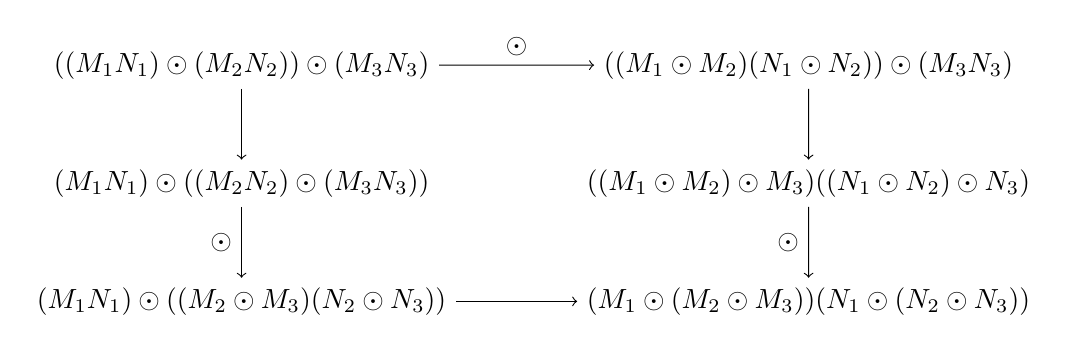
\begin{tikzpicture}[xscale=1.8, yscale=1.5]
\node (tl) at (0,2) {$((M_1 \tens N_1)\odot (M_2 \tens N_2)) \odot (M_3 \tens N_3)$};
\node (tr) at (4,2) {$((M_1 \odot M_2) \tens (N_1 \odot N_2)) \odot (M_3 \tens N_3)$};
\node (ml) at (0,1) {$(M_1 \tens N_1) \odot ((M_2 \tens N_2) \odot (M_3 \tens N_3))$};
\node (mr) at (4,1) {$((M_1 \odot M_2) \odot M_3) \tens ((N_1 \odot N_2) \odot N_3)$};
\node (bl) at (0,0) {$(M_1 \tens N_1) \odot ((M_2 \odot M_3) \tens (N_2 \odot N_3))$};
\node (br) at (4,0) {$(M_1 \odot (M_2 \odot M_3)) \tens (N_1 \odot (N_2 \odot N_3))$};
\draw[->] (tl) to node[above] {$\fx \odot \id$} (tr);
\draw[->] (tl) to node[left]{$\fa$} (ml);
\draw[->] (ml) to node[left]{$\id\odot \fx$} (bl);
\draw[->] (tr) to node[left]{$\fx$} (mr);
\draw[->] (mr) to node[left]{$\fa \odot \fa$} (br);
\draw[->] (bl) to node[above] {$\fx$} (br);
\end{tikzpicture}
    \end{aligned}
\end{equation}

%\begin{equation}\label{eq:mondoub1}
%\begin{aligned}
%  \xymatrix{
%    ((M_1\ten N_1)\odot (M_2\ten N_2)) \odot (M_3\ten N_3) \ar[r]\ar[d]
%    & ((M_1\odot M_2)\ten (N_1\odot N_2)) \odot (M_3\ten N_3) \ar[d]\\
%    (M_1\ten N_1)\odot ((M_2\ten N_2) \odot (M_3\ten N_3)) \ar[d] &
%    ((M_1\odot M_2)\odot M_3) \ten ((N_1\odot N_2)\odot N_3) \ar[d]\\
%    (M_1\ten N_1) \odot ((M_2\odot M_3) \ten (N_2\odot N_3))\ar[r] &
%    (M_1\odot (M_2\odot M_3)) \ten (N_1\odot (N_2\odot N_3))}
%    \end{aligned}
%\end{equation}

\begin{equation}\label{eq:mondoub2}
\begin{aligned}
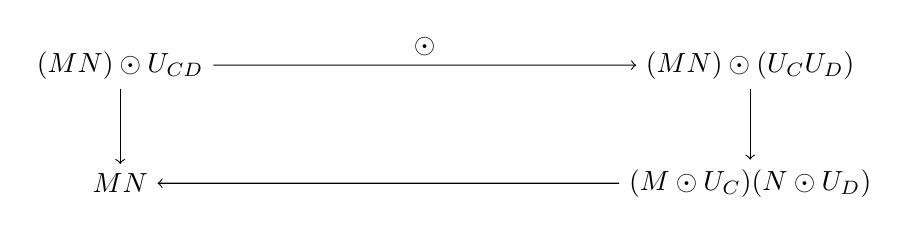
\begin{tikzpicture}[xscale=2, yscale=1.5]
\node (tl) at (0,2) {$(M \tens N) \odot U_{C \tens D}$};
\node (tr) at (4,2) {$(M \tens N) \odot ( U_C \tens U_D)$};
\node (ml) at (0,1) {$M \tens N$};
\node (mr) at (4,1) {$(M \odot U_C) \tens (N \odot U_D)$};
\draw[->] (tl) to node[above] {$\id \odot \fu$} (tr);
\draw[->] (tl) to node[left]{$\fr$} (ml);
\draw[->] (tr) to node[left]{$\fx$} (mr);
\draw[->] (mr) to node[above] {$\fr \tens \fr$} (ml);
\end{tikzpicture}
    \end{aligned}
\end{equation}

%\begin{equation}\label{eq:mondoub2}
%\begin{aligned}    
%  \xymatrix{(M\ten N) \odot U_{C\ten D} \ar[r]\ar[d] &
%    (M\ten N)\odot (U_C\ten U_D) \ar[d]\\
%    M\ten N\ar@{<-}[r] & (M\odot U_C) \ten (N\odot U_D)}
%        \end{aligned}
%    \end{equation}
    
    \begin{equation}\label{eq:mondoub3}
\begin{aligned}
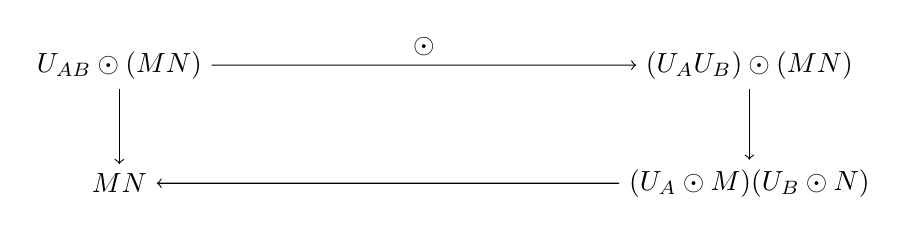
\begin{tikzpicture}[xscale=2, yscale=1.5]
\node (tl) at (0,2) {$U_{A \tens B} \odot (M \tens N) $};
\node (tr) at (4,2) {$(U_A \tens U_B) \odot (M \tens N) $};
\node (ml) at (0,1) {$M \tens N$};
\node (mr) at (4,1) {$(U_A \odot M ) \tens (U_B \odot N)$};
\draw[->] (tl) to node[above] {$\fu \odot \id$} (tr);
\draw[->] (tl) to node[left]{$\fl$} (ml);
\draw[->] (tr) to node[left]{$\fx$} (mr);
\draw[->] (mr) to node[above] {$\fl \tens \fl$} (ml);
\end{tikzpicture}
    \end{aligned}
\end{equation}

%    \begin{equation}\label{eq:mondoub3}
%    \begin{aligned}
%  \xymatrix{U_{A\ten B}\odot (M\ten N)  \ar[r]\ar[d] &
 %   (U_A\ten U_B)\odot (M\ten N) \ar[d]\\
 %   M\ten N\ar@{<-}[r] & (U_A \odot M) \ten (U_B\odot N)}
 %       \end{aligned}
%    \end{equation}
\item \label{eq:mon2}The following diagrams commute, expressing that the
  associativity isomorphism for $\ten$ is a transformation of double
  categories.
\begin{equation}\label{eq:mondoub4}
\begin{aligned}
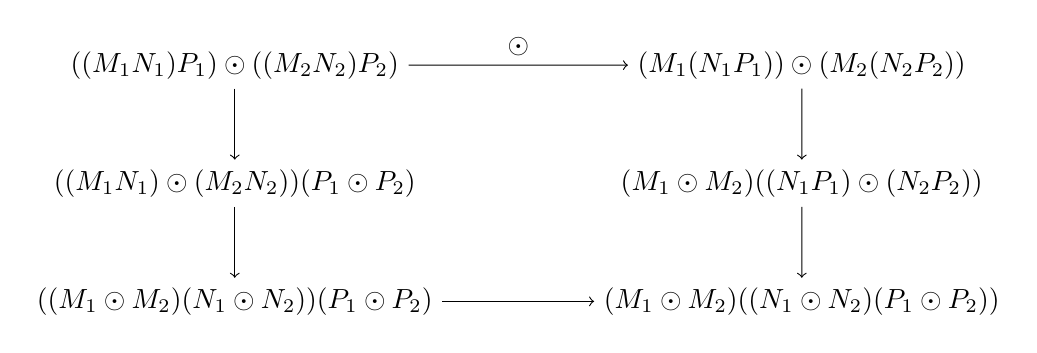
\begin{tikzpicture}[xscale=1.8, yscale=1.5]
\node (tl) at (0,2) {$((M_1 \tens N_1) \tens P_1) \odot ((M_2 \tens N_2) \tens P_2) $};
\node (tr) at (4,2) {$(M_1 \tens (N_1 \tens P_1)) \odot (M_2 \tens (N_2 \tens P_2))$};
\node (ml) at (0,1) {$((M_1 \tens N_1) \odot (M_2 \tens N_2)) \tens (P_1 \odot P_2)$};
\node (mr) at (4,1) {$(M_1 \odot M_2)  \tens ((N_1 \tens P_1) \odot (N_2 \tens P_2))$};
\node (bl) at (0,0) {$((M_1 \odot M_2) \tens (N_1 \odot N_2)) \tens (P_1 \odot P_2)$};
\node (br) at (4,0) {$(M_1 \odot M_2) \tens ((N_1 \odot N_2) \tens (P_1 \odot P_2))$};
\draw[->] (tl) to node[above] {$\fa \odot \fa$} (tr);
\draw[->] (tl) to node[left]{$\fx$} (ml);
\draw[->] (ml) to node[left]{$ \fx \tens \id$} (bl);
\draw[->] (tr) to node[left]{$\fx$} (mr);
\draw[->] (mr) to node[left]{$\id \tens \fx$} (br);
\draw[->] (bl) to node[above] {$\fa$} (br);
\end{tikzpicture}
    \end{aligned}
\end{equation}
  
%     {\small 
%\begin{equation}\label{eq:mondoub4}
%\begin{aligned}
%  \xymatrix{
%    ((M_1\ten N_1)\ten P_1) \odot ((M_2\ten N_2)\ten P_2) \ar[r]\ar[d] &
 %   (M_1\ten (N_1\ten P_1)) \odot (M_2\ten (N_2\ten P_2)) \ar[d]\\
    %((M_1\ten N_1) \odot (M_2\ten N_2)) \ten (P_1\odot P_2) \ar[d] &
%    (M_1\odot M_2) \ten ((N_1\ten P_1)\odot (N_2\ten P_2))\ar[d] \\
   % ((M_1\odot M_2) \ten(N_1\odot N_2)) \ten (P_1\odot P_2) \ar[r] &
%    (M_1\odot M_2) \ten ((N_1\odot N_2)\ten (P_1\odot P_2))}
   %     \end{aligned}
      %  \end{equation}
        
        \begin{equation}\label{eq:mondoub5}
\begin{aligned}
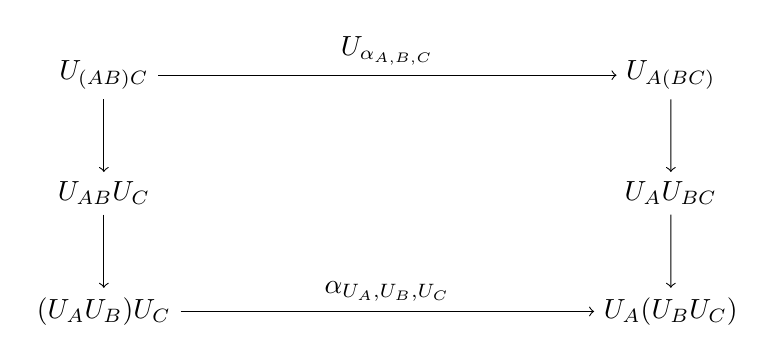
\begin{tikzpicture}[xscale=1.8, yscale=1.5]
\node (tl) at (0,2) {$U_{(A \tens B) \tens C}$};
\node (tr) at (4,2) {$U_{A \tens (B \tens C)}$};
\node (ml) at (0,1) {$U_{A \tens B} \tens U_C$};
\node (mr) at (4,1) {$U_A \tens U_{B \tens C}$};
\node (bl) at (0,0) {$(U_A \tens U_B) \tens U_C$};
\node (br) at (4,0) {$U_A \tens (U_B \tens U_C)$};
\draw[->] (tl) to node[above] {$U_{\alpha_{A,B,C}}$} (tr);
\draw[->] (tl) to node[left]{$\fu$} (ml);
\draw[->] (ml) to node[left]{$\fu \tens \id$} (bl);
\draw[->] (tr) to node[left]{$\fu$} (mr);
\draw[->] (mr) to node[left]{$\id \tens \fu$} (br);
\draw[->] (bl) to node[above] {$\alpha_{U_A, U_B, U_C}$} (br);
\end{tikzpicture}
    \end{aligned}
\end{equation}
%    \begin{equation}\label{eq:mondoub5}
  %  \begin{aligned}
  %\xymatrix{
%    U_{(A\ten B)\ten C} \ar[r] \ar[d] & U_{A\ten (B\ten C)} \ar[d]\\
   % U_{A\ten B} \ten U_C \ar[d] & U_A\ten U_{B\ten C}\ar[d]\\
%    (U_A\ten U_B)\ten U_C \ar[r] & U_A\ten (U_B\ten U_C) }
   %     \end{aligned}
   % \end{equation}
    %}

\item \label{eq:mon3}The following diagrams commute, expressing that the unit
  isomorphisms for $\ten$ are transformations of double categories.
 \begin{equation}\label{eq:mondoub6}
\begin{aligned}
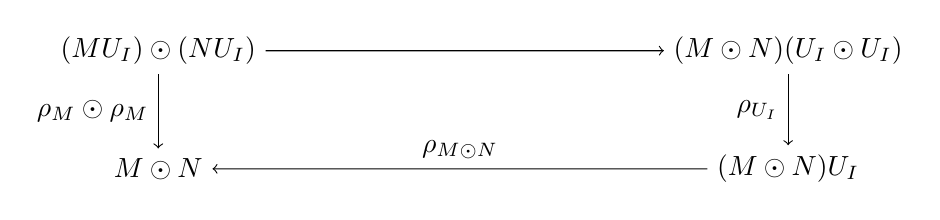
\begin{tikzpicture}[xscale=2, yscale=1.5]
\node (tl) at (0,2) {$(M \tens U_I) \odot (N \tens U_I) $};
\node (tr) at (4,2) {$(M \odot N) \tens ( U_I \odot U_I)$};
\node (ml) at (0,1) {$M \odot N$};
\node (mr) at (4,1) {$(M \odot N) \tens U_I$};
\draw[->] (tl) to node[above] {$\fx$} (tr);
\draw[->] (tl) to node[left]{$\rho_M \odot \rho_M$} (ml);
\draw[->] (tr) to node[left]{$\id \tens \rho_{U_I}$} (mr);
\draw[->] (mr) to node[above] {$\rho_{M \odot N}$} (ml);
\end{tikzpicture}
    \end{aligned}
\end{equation}
      
      \begin{equation}\label{eq:mondoub7}
\begin{aligned}
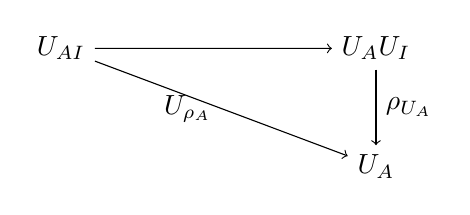
\begin{tikzpicture}[yscale=1.5]
\node (tl) at (0,2) {$U_{A\tens I}$};
\node (tr) at (4,2) {$U_A \tens  U_I$};
\node (mr) at (4,1) {$U_A$};
\draw[->] (tl) to node[above]{$\fu$} (tr);
\draw[->] (tl) to node[left]{$U_{\rho_A}$} (mr);
\draw[->] (tr) to node[right]{$\rho_{U_A}$} (mr);
\end{tikzpicture}
    \end{aligned}
\end{equation}

 \begin{equation}\label{eq:mondoub8}
\begin{aligned}
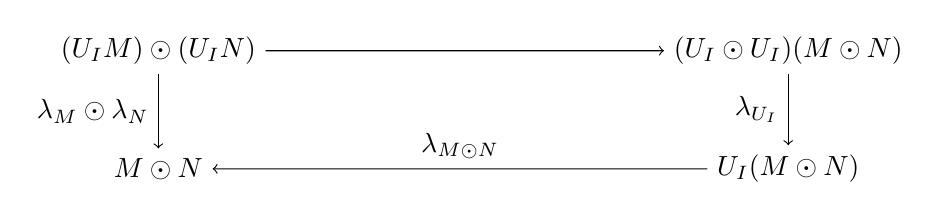
\begin{tikzpicture}[xscale=2, yscale=1.5]
\node (tl) at (0,2) {$(U_I \tens M) \odot ( U_I \tens N) $};
\node (tr) at (4,2) {$( U_I \odot U_I) \tens (M \odot N) $};
\node (ml) at (0,1) {$M \odot N$};
\node (mr) at (4,1) {$U_I \tens (M \odot N) $};
\draw[->] (tl) to node[above] {$\fx$} (tr);
\draw[->] (tl) to node[left]{$\lambda_M \odot \lambda_N$} (ml);
\draw[->] (tr) to node[left]{$\lambda_{U_I} \tens \id$} (mr);
\draw[->] (mr) to node[above] {$\lambda_{M \odot N}$} (ml);
\end{tikzpicture}
    \end{aligned}
\end{equation}
      
      \begin{equation}\label{eq:mondoub9}
\begin{aligned}
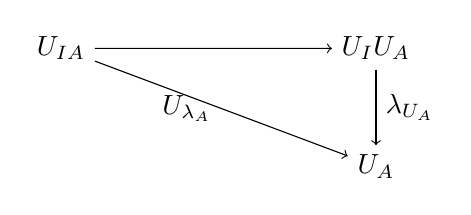
\begin{tikzpicture}[yscale=1.5]
\node (tl) at (0,2) {$U_{I\tens A}$};
\node (tr) at (4,2) {$U_I \tens  U_A$};
\node (mr) at (4,1) {$U_A$};
\draw[->] (tl) to node[above]{$\fu$} (tr);
\draw[->] (tl) to node[left]{$U_{\lambda_A}$} (mr);
\draw[->] (tr) to node[right]{$\lambda_{U_A}$} (mr);
\end{tikzpicture}
    \end{aligned}
\end{equation}

  \setcounter{mondbl}{\value{enumi}}
\end{enumerate}
Similarly, a \textbf{braided monoidal double category} is a monoidal double
category with the following additional structure.
\begin{enumerate}\setcounter{enumi}{\value{mondbl}}
\item $\lD_0$ and $\lD_1$ are braided monoidal categories.
\item The functors $S$ and $T$ are strict braided monoidal (i.e.\ they
  preserve the braidings).
\item \label{eq:braid1} The following diagrams commute, expressing that the braiding is
  a transformation of double categories. 
  \begin{equation}\label{eq:brmondoub1}
\begin{aligned}
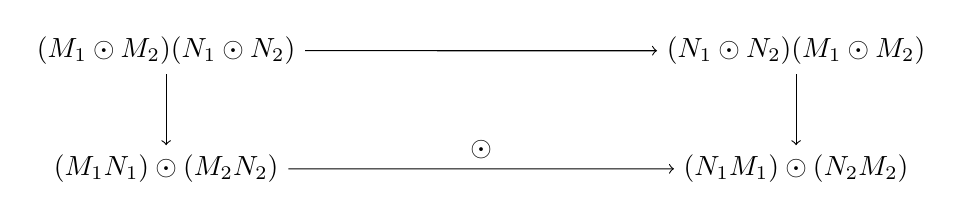
\begin{tikzpicture}[xscale=2, yscale=1.5]
\node (tl) at (0,2) {$(M_1 \odot M_2) \tens (N_1 \odot N_2)$};
\node (tr) at (4,2) {$(N_1 \odot N_2) \tens (M_1 \odot M_2)$};
\node (ml) at (0,1) {$(M_1 \tens N_1) \odot (M_2 \tens N_2)$};
\node (mr) at (4,1) {$(N_1 \tens M_1) \odot (N_2 \tens M_2)$};
\draw[->] (tl) to node[above] {$\fs$} (tr);
\draw[->] (tl) to node[left]{$\fx$} (ml);
\draw[->] (tr) to node[left]{$\fx$} (mr);
\draw[->] (ml) to node[above] {$\fs \odot \fs$} (mr);
\end{tikzpicture}
    \end{aligned}
\end{equation}
  %\[\xymatrix{(M_1\odot M_2)\ten (N_1\odot N_2) \ar[r]^\fs\ar[d]_\fx &
  %  (N_1\odot N_2)\ten (M_1 \odot M_2)\ar[d]^\fx\\
   % (M_1\ten N_1)\odot (M_2\ten N_2) \ar[r]_{\fs\odot \fs} &
  %  (N_1\ten M_1) \odot (N_2 \ten M_2)}
 % \]
 \begin{equation}\label{eq:brmondoub2}
\begin{aligned}
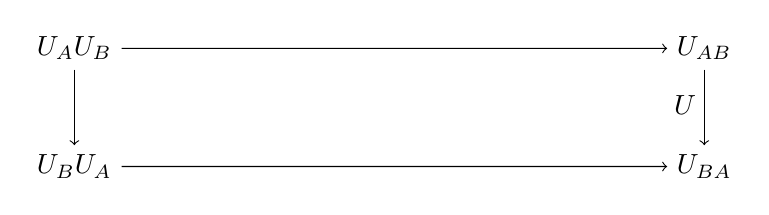
\begin{tikzpicture}[xscale=2, yscale=1.5]
\node (tl) at (0,2) {$U_A \tens U_B$};
\node (tr) at (4,2) {$U_{A \tens B}$};
\node (ml) at (0,1) {$U_B \tens U_A$};
\node (mr) at (4,1) {$U_{B \tens A}$};
\draw[->] (tl) to node[above] {$\fu$} (tr);
\draw[->] (tl) to node[left]{$\fs$} (ml);
\draw[->] (tr) to node[left]{$U_{\fs}$} (mr);
\draw[->] (ml) to node[above] {$\fu$} (mr);
\end{tikzpicture}
    \end{aligned}
\end{equation}

 % \[\xymatrix{U_A \ten U_B \ar[r]^(0.55)\fu \ar[d]_\fs &
  %  U_{A\ten B} \ar[d]^{U_\fs}\\
  %  U_B\ten U_A \ar[r]_(0.55)\fu &
  %  U_{B\ten A}}.
  %\]
  \setcounter{mondbl}{\value{enumi}}
\end{enumerate}
Finally, a \textbf{symmetric monoidal double category} is a braided one such that
\begin{enumerate}\setcounter{enumi}{\value{mondbl}}
\item $\lD_0$ and $\lD_1$ are in fact symmetric monoidal.
\end{enumerate}
While there are a fair number of coherence diagrams in this definition, most of
them are fairly small, and in any given case most or all of them are
fairly obvious.  Thus, verifying that a given double category is
(braided or symmetric) monoidal is not a great deal of work.

%\fxnote[author=LW]{If we merge the examples with the final section, this should be included.}
\begin{eg}
  The examples \lMod, \lnCob, and \lProf\ are all easily seen to be
  symmetric monoidal under the tensor product of rings, disjoint union
  of manifolds, and cartesian product of categories, respectively.
\end{eg}

\begin{rmk}
  In a 2-category with finite products there is additionally the
  notion of a \emph{cartesian object}: one such that the diagonal
  $D\to D\times D$ and projection $D\to 1$ have right adjoints.  Any
  cartesian object is a symmetric pseudomonoid in a canonical way,
  just as any category with finite products is a monoidal category
  with its cartesian product.  Many of the ``cartesian bicategories''
  considered in~\cite{cw:cart-bicats-i,ckww:cartbicats-ii} are in
  fact the loose bicategory of some cartesian object in \cDbl,
  and inherit their monoidal structure in this way.
  Cartesian double categories have recently been further studied by~\cite{aleiferi2018cartesian}.
\end{rmk}

Two further general methods for constructing symmetric monoidal double
categories can be found in~\cite{shulman:frbi}.

\begin{rmk}
  The general yoga of internalization says that an $X$ internal to
  $Y$s internal to $Z$s is equivalent to a $Y$ internal to $X$s
  internal to $Z$s, but this is only strictly true when the
  internalizations are all strict.  We have defined a symmetric
  monoidal double category to be a (pseudo) symmetric monoid internal
  to (pseudo) categories internal to categories, but one could also
  consider a (pseudo) category internal to (pseudo) symmetric monoids
  internal to categories, i.e.\ a pseudo internal category in the
  2-category
  $\mathcal{S}\mathit{ym}\mathcal{M}\mathit{on}\mathcal{C}\mathit{at}$
  of symmetric monoidal categories and strong symmetric monoidal
  functors.  This would give \emph{almost} the same definition, except
  that $S$ and $T$ would only be strong monoidal (preserving $\ten$ up
  to isomorphism) rather than strict monoidal.  We prefer our
  definition, since $S$ and $T$ are strict monoidal in almost all
  examples, and keeping track of their constraints would be tedious.
\end{rmk}

Just as every bicategory is equivalent to a strict 2-category, it is
proven in~\cite{gp:double-limits} that every pseudo double category is
equivalent to a strict double category (one in which the associativity
and unit constraints for $\odot$ are identities).  Thus, from now on
we will usually omit to write these constraint isomorphisms (or
equivalently, implicitly strictify our double categories).  We
\emph{will} continue to write the constraint isomorphisms for the
monoidal structure $\ten$, since these are where the whole question
lies.

We now move on to define functors and transformations of monoidal double categories.
Like monoidal double categories themselves, these are also special cases of a notion that makes sense internal to any 2-category with products.

\begin{defn}\label{def:monfunc}
  Let $\D$, $\E$ be (braided/symmetric) monoidal double categories.  A {\bf (braided or symmetric) lax monoidal double functor} $F: \D \rightarrow \E$ is a pseudo double functor $F$, together with transformations $\phi : \otimes \circ (F,F) \rightarrow F \circ \otimes$ and $\phi_u:I_{\E}\rightarrow F \circ I_{\D}$ satisfying the usual axioms for (braided/symmetric) monoidal functors with respect to $\otimes$.
\end{defn}

Unfolding the definitions gives us:

\begin{enumerate}
\item $F_0$ and $F_1$ are (braided/symmetric) monoidal functors.
\item The equalities $F_0 \circ S_\D = S_\E \circ F_1$ and $F_0 \circ T_\D = T_\E \circ F_1$ are strict equalities of monoidal functors.
\item The following diagrams commute, expressing that $\phi$ is a transformation of double categories:

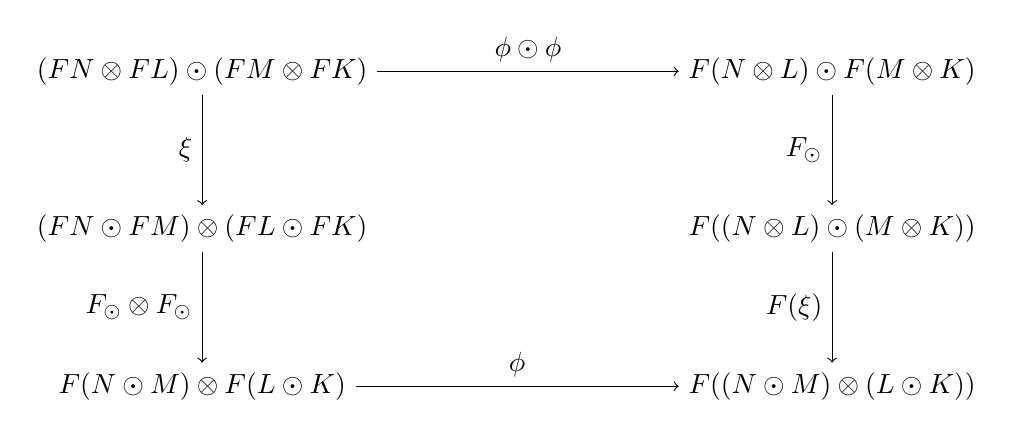
\begin{tikzpicture}[xscale=2, yscale=2]
\node (tl) at (0,2) {$(FN \otimes FL) \odot (FM \otimes FK)$};
\node (tr) at (4,2) {$F(N\otimes L) \odot F(M \otimes K)$};
\draw[->] (tl) to node[above] {$\phi \odot \phi$} (tr);
\node (ml) at (0,1) {$(FN \odot FM) \otimes (FL \odot FK)$};
\node (mr) at (4,1) {$F((N \otimes L) \odot (M \otimes K))$};
\node (bl) at (0,0) {$F(N \odot M) \otimes F(L \odot K)$};
\node (br) at (4,0) {$F((N \odot M)\otimes(L\odot K))$};
\draw[->] (tl) to node[left]{$\xi$} (ml);
\draw[->] (ml) to node[left]{$F_{\odot} \otimes F_{\odot}$} (bl);
\draw[->] (tr) to node[left]{$F_{\odot}$} (mr);
\draw[->] (mr) to node[left]{$F(\xi)$} (br);
\draw[->] (bl) to node[above] {$\phi$} (br);
\end{tikzpicture}

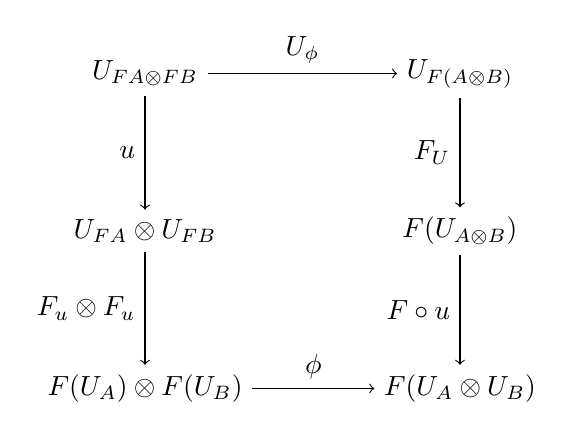
\begin{tikzpicture}[yscale=2]
\node (tl) at (0,2) {$U_{FA \otimes FB}$};
\node (tr) at (4,2) {$U_{F(A \otimes B)} $};
\draw[->] (tl) to node[above] {$U_{\phi}$} (tr);
\node (ml) at (0,1) {$U_{FA} \otimes U_{FB}$};
\node (mr) at (4,1) {$F(U_{A\otimes B}) $};
\node (bl) at (0,0) {$F(U_A) \otimes F(U_B)$};
\node (br) at (4,0) {$F(U_A \otimes U_B)$};
\draw[->] (tl) to node[left]{$u$} (ml);
\draw[->] (ml) to node[left]{$F_u \otimes F_u$} (bl);
\draw[->] (tr) to node[left]{$F_U$} (mr);
\draw[->] (mr) to node[left]{$F \circ u$} (br);
\draw[->] (bl) to node[above] {$\phi$} (br);
\end{tikzpicture}

\end{enumerate}

When the natural transformations are in the opposite direction, the functor is {\bf colax monoidal}, and when they are isomorphisms, the functor is {\bf strong monoidal}.

\begin{defn}\label{Def:monverttrans}
  Let $\D$, $\E$ be monoidal double categories and let $(F, \phi) ,(G,\psi): \D \rightarrow \E$ be monoidal double functors. A \textbf{monoidal transformation} $\alpha: F \rightarrow G$ is a tight transformation such that $\alpha_0$ and $\alpha_1$ are monoidal natural transformations.
  Explicitly, this means (in the lax case) that the following equalities hold:

\begin{equation}
\begin{aligned}
\begin{tikzpicture}
\node (tl) at (0,4) {$FA \otimes FB$};
\node (tr) at (4,4) {$FC \otimes FD$};
\node (ml) at (0,2) {$F(A\otimes B)$};
\node (mr) at (4,2) {$F(C \otimes D)$};
\node (bl) at (0,0) {$G(A \otimes B)$};
\node (br) at (4,0) {$G(C \otimes D)$};
\draw[style=tickarrow] (tl) to node [above] {$FM \otimes FN$} (tr);
\draw[style=tickarrow] (ml) to node [above] {$F(M\otimes N)$} (mr);
\draw[->] (tl) to node [left] {$\phi_{A,B}$} (ml);
\draw[->] (tr) to node [right] {$\phi_{C,D}$}(mr);
\draw[->] (ml) to node [left] {$\alpha_{A\otimes B}$} (bl);
\draw[->] (mr) to node [right] {$\alpha_{C \otimes D}$} (br);
\draw[style=tickarrow] (bl) to node [above] {$G(M \otimes N)$} (br);
\node at (2,3) {$\Downarrow \phi_{M,N}$};
\node at (2,1) {$\Downarrow \alpha_{M \otimes N}$};
\end{tikzpicture}
\end{aligned}
=
\begin{aligned}
\begin{tikzpicture}
\node (tl) at (0,4) {$FA \otimes FB$};
\node (tr) at (4,4) {$FC \otimes FD$};
\node (ml) at (0,2) {$GA \otimes GB$};
\node (mr) at (4,2) {$GC \otimes GD$};
\node (bl) at (0,0) {$G(A \otimes B)$};
\node (br) at (4,0) {$G(C \otimes D)$};
\draw[style=tickarrow] (tl) to node [above] {$FM \otimes FN$} (tr);
\draw[style=tickarrow] (ml) to node [above] {$GM \otimes GN$} (mr);
\draw[->] (tl) to node [left] {$\alpha_A \otimes \alpha_B$} (ml);
\draw[->] (tr) to node [right] {$\alpha_C \otimes \alpha_D$} (mr);
\draw[->] (ml) to node [left] {$\psi_{A,B}$} (bl);
\draw[->] (mr) to node [right] {$\psi_{C,D}$} (br);
\draw[style=tickarrow] (bl) to node [above] {$G(M \otimes N)$} (br);
\node at (2,3) {$\Downarrow \alpha_M \otimes \alpha_N$};
\node at (2,1) {$\Downarrow \psi_{M,N}$};
\end{tikzpicture}
\end{aligned}
\end{equation}

\begin{equation}
\begin{aligned}
\begin{tikzpicture}
\node (tl) at (0,4) {$I_{\mathbb{E}}$};
\node (tr) at (4,4) {$I_{\mathbb{E}}$};
\node (ml) at (0,2) {$F(I_{\mathbb{D}})$};
\node (mr) at (4,2) {$F(I_{\mathbb{D}})$};
\node (bl) at (0,0) {$G(I_{\mathbb{D}})$};
\node (br) at (4,0) {$G(I_{\mathbb{D}})$};
\draw[style=tickarrow] (tl) to node [above] {$U_{I_{\mathbb{E}}}$} (tr);
\draw[style=tickarrow] (ml) to node [above] {$F(U_{I_{\mathbb{D}}})$} (mr);
\draw[->] (tl) to node [left] {$\phi_{u_0}$} (ml);
\draw[->] (tr) to node [right] {$\phi_{u_1}$}(mr);
\draw[->] (ml) to node [left] {$\alpha_{I_{\mathbb{D}}}$} (bl);
\draw[->] (mr) to node [right] {$\alpha_{I_{\mathbb{D}}}$} (br);
\draw[style=tickarrow] (bl) to node [below] {$G(U_{I_{\mathbb{D}}})$} (br);
\node at (2,3) {$\Downarrow \phi_{u_1}$};
\node at (2,1) {$\Downarrow \alpha_{U_{I_{\mathbb{D}}}}$};
\end{tikzpicture}
\end{aligned}
=
\begin{aligned}
\begin{tikzpicture}
\node (tl) at (0,4) {$I_{\mathbb{E}}$};
\node (tr) at (4,4) {$I_{\mathbb{E}}$};
\node (ml) at (0,2) {$G(I_{\mathbb{D}})$};
\node (mr) at (4,2) {$G(I_{\mathbb{D}})$};
\draw[style=tickarrow] (tl) to node [above] {$U_{I_{\mathbb{E}}}$} (tr);
\draw[style=tickarrow] (ml) to node [below] {$G(U_{I_{\mathbb{D}}})$} (mr);
\draw[->] (tl) to node [left] {$\psi_{u}$} (ml);
\draw[->] (tr) to node [right] {$\psi_{u}$}(mr);
\node at (2,3) {$\Downarrow \psi_{u_1}$};
\end{tikzpicture}
\end{aligned}
\end{equation}


A {\bf braided or symmetric monoidal tight transformation} is a monoidal transformation between braided/symmetric monoidal functors.
\end{defn}

We have three strict 2-categories $\cMonDbll, \cMonDblc,\cMonDblp$ of monoidal double categories and lax, colax, or pseudo monoidal functors, respectively.
(More generally, we have three such 2-categories of pseudomonoids internal to any 2-category with finite products.)


% Local Variables:
% TeX-master: "smbicat"
% End:
